\documentclass[supercite]{Experimental_Report}

\title{~~~~~~新生实践课~~~~~~}
\author{董哲}
\school{计算机科学与技术学院}
\classnum{CS2408}
\stunum{U202414746}
\instructor{李蓉} % 李平、孙伟平、范晔斌、陈加忠
\date{2024年11月11日}

\usepackage{algorithm, multirow}
\usepackage{algpseudocode}
\usepackage{amsmath}
\usepackage{amsthm}
\usepackage{framed}
\usepackage{mathtools}
\usepackage{subcaption}
\usepackage{xltxtra} %提供了针对XeTeX的改进并且加入了XeTeX的LOGO, 自动调用xunicode宏包(提供Unicode字符宏)
\usepackage{bm}
\usepackage{tikz}
\usepackage{tikzscale}
\usepackage{pgfplots}
%\usepackage{enumerate}

\pgfplotsset{compat=1.16}

\newcommand{\cfig}[3]{
  \begin{figure}[htb]
    \centering
    \includegraphics[width=#2\textwidth]{images/#1.tikz}
    \caption{#3}
    \label{fig:#1}
  \end{figure}
}

\newcommand{\sfig}[3]{
  \begin{subfigure}[b]{#2\textwidth}
    \includegraphics[width=\textwidth]{images/#1.tikz}
    \caption{#3}
    \label{fig:#1}
  \end{subfigure}
}

\newcommand{\xfig}[3]{
  \begin{figure}[htb]
    \centering
    #3
    \caption{#2}
    \label{fig:#1}
  \end{figure}
}

\newcommand{\rfig}[1]{\autoref{fig:#1}}
\newcommand{\ralg}[1]{\autoref{alg:#1}}
\newcommand{\rthm}[1]{\autoref{thm:#1}}
\newcommand{\rlem}[1]{\autoref{lem:#1}}
\newcommand{\reqn}[1]{\autoref{eqn:#1}}
\newcommand{\rtbl}[1]{\autoref{tbl:#1}}

\algnewcommand\Null{\textsc{null }}
\algnewcommand\algorithmicinput{\textbf{Input:}}
\algnewcommand\Input{\item[\algorithmicinput]}
\algnewcommand\algorithmicoutput{\textbf{Output:}}
\algnewcommand\Output{\item[\algorithmicoutput]}
\algnewcommand\algorithmicbreak{\textbf{break}}
\algnewcommand\Break{\algorithmicbreak}
\algnewcommand\algorithmiccontinue{\textbf{continue}}
\algnewcommand\Continue{\algorithmiccontinue}
\algnewcommand{\LeftCom}[1]{\State $\triangleright$ #1}

\newtheorem{thm}{定理}[section]
\newtheorem{lem}{引理}[section]

\colorlet{shadecolor}{black!15}

\theoremstyle{definition}
\newtheorem{alg}{算法}[section]

\def\thmautorefname~#1\null{定理~#1~\null}
\def\lemautorefname~#1\null{引理~#1~\null}
\def\algautorefname~#1\null{算法~#1~\null}

\begin{document}

\maketitle

\clearpage

\pagenumbering{Roman}

\tableofcontents[level=2]
\clearpage

\pagenumbering{arabic}

\section{网页整体框架}
首先确定主题——自我介绍。

然后是是网页整体框架——图\ref{fig1-1},由一个主页面及下面的四个分页面组成。网页间的跳转并没有使用超链接的形式,而是使用了一种更难的方式——将四个分页面置于四个<section>元素,每个section元素都有一个向下的箭头图标,通过js代码实现用于滚动到下一个section,提供了一定的交互性。



\begin{figure}[htb] % here top bottom
	\begin{center}
		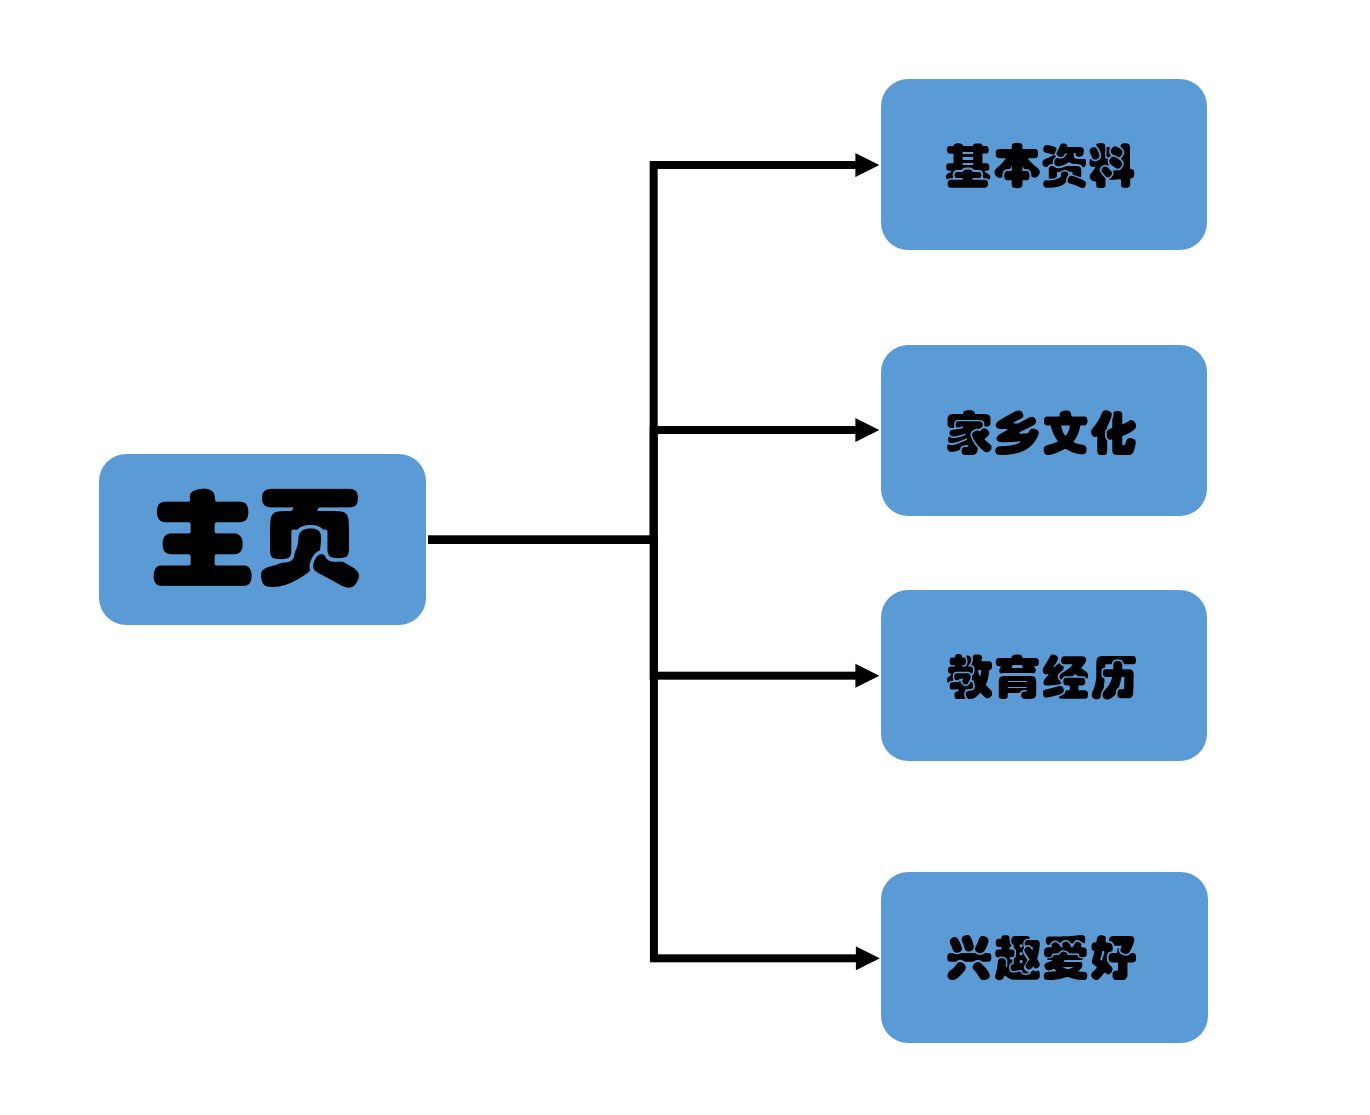
\includegraphics[scale=0.10]{images/1-1.png}
		\caption{网页整体框架}
		\label{fig1-1}
	\end{center}
\end{figure}



\begin{enumerate}
\renewcommand{\labelenumi}{\theenumi)}
	\item 主页
	\item 基本资料
	\item 家乡文化
        \item 教育经历
        \item 兴趣爱好
\end{enumerate}

\begin{figure}[htb]
	\begin{center}
		\includegraphics[scale=0.20]{images/1-2.png}
		\caption{主页效果}
		\label{fig1-2}
	\end{center}
\end{figure}




\newpage

\section{主页设计}
\begin{enumerate}
\renewcommand{\labelenumi}{\theenumi)}
	\item 为了便于跳转,在各个section部分设置锚点
	
	\item 为了好玩,当鼠标移动到图片上时,通过更换src属性实现更换图片
\end{enumerate}


\begin{figure}[htb]
	\begin{center}
		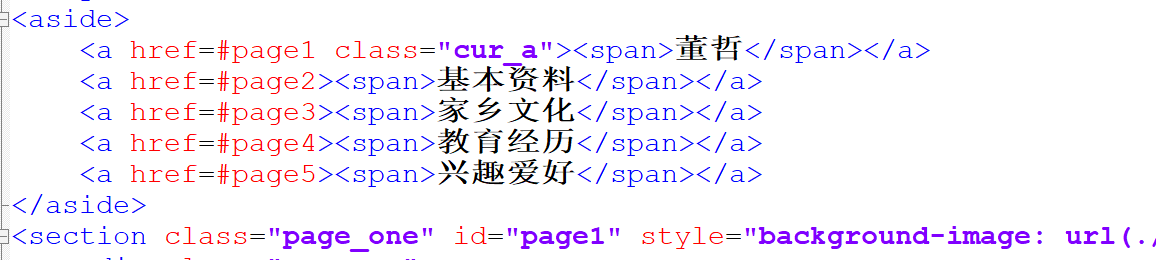
\includegraphics[scale=0.40]{images/2-1.png}
		\caption{主页代码举例}
		\label{fig2-1}
	\end{center}
\end{figure}

通过在<section>部分设置id=page1,同时在主页用超链接”href=page1“实现同一页面的跳转。并设置属性onmousewheel="return false;“,禁止鼠标滚动。

\begin{figure}[htb]
	\begin{center}
		
\includegraphics[scale=0.40]{images/2-2.png}
		\caption{主页代码举例}
		\label{fig2-2}
	\end{center}
\end{figure}

<img onmousemove="this.src='./end.png'" onmouseout="this.src='./start.png'">:这是一个图片元素,src="./start.png":指定了图片的初始源文件路径,即页面加载时显示的图片是start.png。

onmousemove="this.src='./end.png'":当鼠标在图片上移动时,会触发这个 JavaScript 事件处理函数,它会将图片的src属性更改为end.png,从而实现鼠标移动到图片上时更换图片的效果。

onmouseout="this.src='./start.png'":当鼠标移出图片时,会触发这个事件处理函数,将图片的src属性重新设置为start.png,恢复到初始图片显示状态。



\newpage

\section{分页面设计}

\subsection{页面1 基本资料}

\begin{figure}[htb]
	\begin{center}
		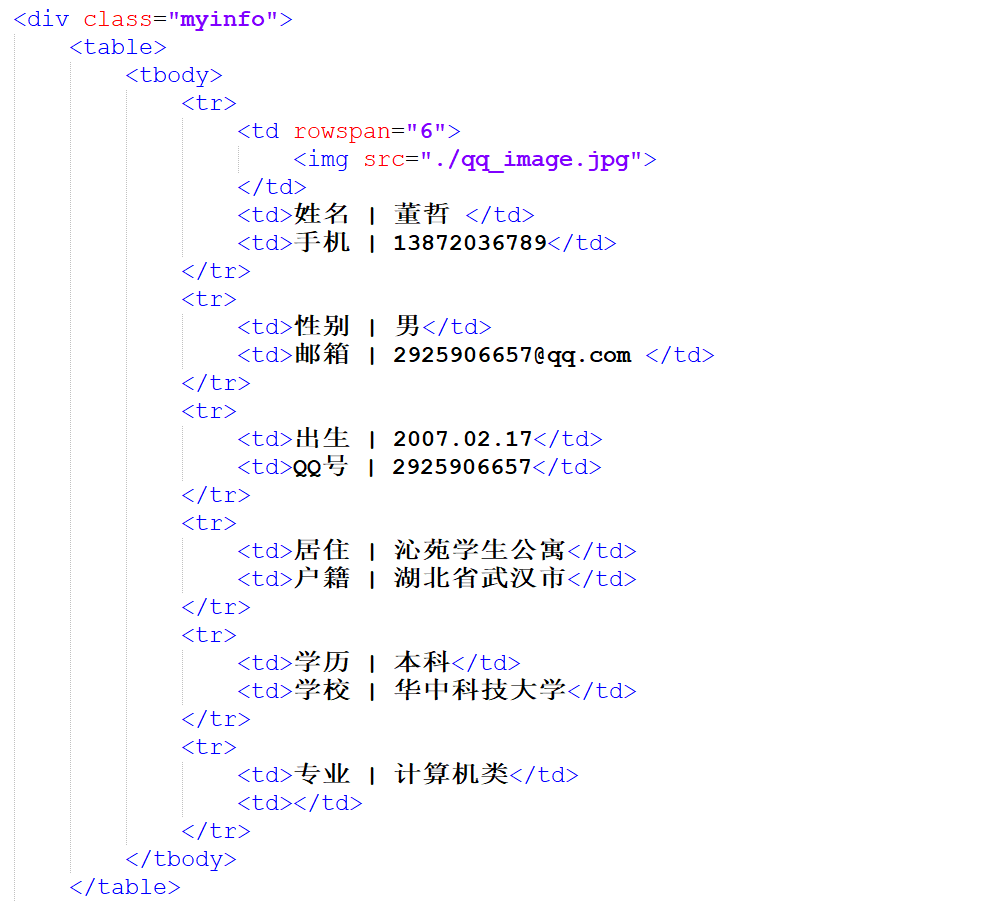
\includegraphics[scale=0.40]{images/3-1.png}
		\caption{代码举例}
		\label{fig3-1}
	\end{center}
\end{figure}


<div class="tit-wrap">:是一个容器<div>,用于对其内部的标题和相关描述内容进行组织。<h1 style="font-weight: bold; text-align: center;">基本资料</h1>:这是一个一级标题元素<h1>,通过内联样式设置了字体加粗(font-weight: bold)并且文本居中(text-align: center),用于突出显示 “基本资料” 这个主题内容。<div class="scissors" style="border-top:1px dashed orange;">:这是一个用于创建视觉分隔效果的<div>元素。通过设置border-top:1px dashed orange;的内联样式,为其顶部添加了一条 1 像素宽样式的边框。<h2 style="text-align: center;">

<table>元素用于创建一个表格。<tbody>标签用于包裹表格的主体内容,将表格的行(<tr>)和列(<td>)内容组织在一起。<tr>标签表示表格的行。这里有多行用于展示不同方面的个人信息。<td rowspan="6">:这是表格中的一个单元格(<td>),设置了rowspan="6"属性,意味着这个单元格将垂直跨越 6 行。其他的<td>单元格用于展示诸如姓名、性别、手机、邮箱等各种个人基本信息,每个<td>单元格对应表格中的一列数据,通过与不同行的组合来完整呈现个人信息的表格内容。


\subsection{页面2 家乡文化}

\begin{figure}[htb]
	\begin{center}
		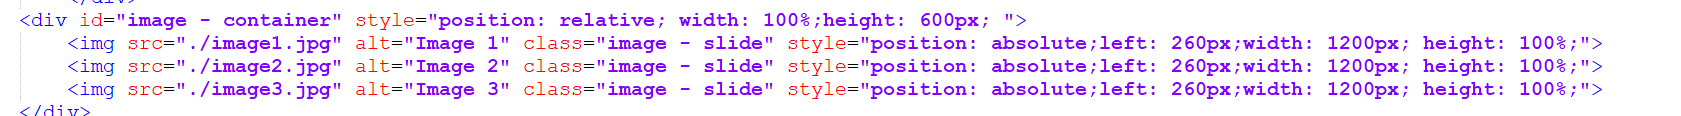
\includegraphics[scale=0.30]{images/4-1.png}
		\caption{html部分}
		\label{fig4-1}
	\end{center}
\end{figure}



\begin{figure}[htb]
	\begin{center}
		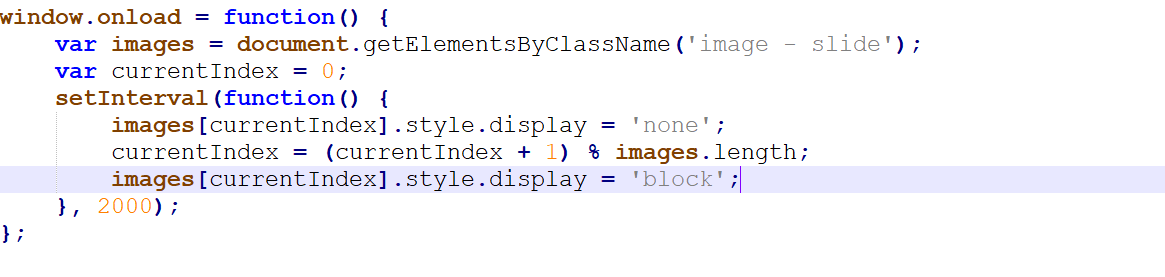
\includegraphics[scale=0.40]{images/4-2.png}
		\caption{css部分}
		\label{fig4-2}
	\end{center}
\end{figure}

window.onload = function() {... }:这是一个 JavaScript 的事件处理函数,它会在页面加载完成后被执行。var images = document.getElementsByClassName('image-slide');:在函数内部,首先通过document.getElementsByClassName('image-slide')方法获取到了所有具有image-slide类名的元素,在这里就是前面 HTML 部分中定义的那三张图片元素,将它们存储在变量images中,以便后续对这些图片进行操作。images[currentIndex].style.display = 'none';首先,通过images[currentIndex]找到当前索引位置(由currentIndex变量指定)的图片元素,然后将其style.display属性设置为none,这会使该图片隐藏起来,不再在页面上显示。

currentIndex = (currentIndex + 1)  images.length;更新currentIndex变量的值。这里先将currentIndex加 1,然后通过取模运算确保它的值始终在images.length(即图片的总数,这里是 3)的范围内。例如,当currentIndex为 2(即最后一张图片)时,加 1 后变为 3,再取模 3 得到 0,这样就实现了循环切换图片的索引位置,保证可以在三张图片之间循环切换。images[currentIndex].style.display = 'block';最后,根据更新后的currentIndex值找到新的图片元素,并将其style.display属性设置为block,使这张新的图片显示在页面上。





\subsection{页面3 教育经历}

没什么好说的,只是一些背景,字体,格式的控制。


\begin{figure}[htb]
	\begin{center}
		
\includegraphics[scale=0.25]{images/5-1.png}
		\caption{效果如图}
		\label{fig5-1}
	\end{center}
\end{figure}

\subsection{页面4 兴趣爱好}

简单介绍一下兴趣,尝试多种字体。

\begin{figure}[htb]
	\begin{center}
		
\includegraphics[scale=0.25]{images/6-1.png}
		\caption{效果如图}
		\label{fig6-1}
	\end{center}
\end{figure}

\newpage

\section{网页设计小结}

在本次网页设计过程中,遇到不少困难。交互上,复杂功能如图片轮播的 JavaScript 逻辑编写困难,与后端数据交互存在数据处理和安全问题。
针对布局,用媒体查询和相对单位调整样式,借助 CSS 框架处理兼容性。
通过此次设计,我掌握了网页设计核心技术,提升了解决问题与编程能力。

\newpage

\section{课程的收获和建议}

在本次网页设计历程中,我遭遇了诸多棘手难题。于视觉设计环节,色彩搭配的协调性难以把控,选定的色调组合在页面呈现时显得突兀杂乱,无法营造出预期的和谐氛围与视觉焦点。同时,图标设计与整体风格的融合也颇具挑战,自制图标在风格上难以与页面的主题和文字排版相得益彰,影响了页面的整体美感与专业性。
在前端开发阶段,HTML 结构的组织不够清晰高效,导致代码冗余,后期维护和修改极为不便。CSS 样式的优先级管理容易混乱,使得某些样式规则相互冲突,元素的样式呈现出错。而 JavaScript 函数的调用顺序和作用域问题也频繁引发错误,致使交互功能的实现出现障碍。
为攻克这些难关,我反复调试色彩比例,实现了较为舒适的视觉效果。针对图标问题,精心挑选适配风格的开源图标或重新设计,确保风格统一。在前端代码方面,重新规划 HTML 结构,遵循语义化原则,运用 CSS 预处理器合理管理样式优先级,仔细梳理 JavaScript 函数逻辑与作用域,借助调试工具逐步排查错误。
经此一役,我大幅提升了网页设计与开发技能,对视觉美感和代码规范有了更深领悟。日后,我期盼能深入探究前沿设计趋势,如响应式动效设计,持续优化代码性能,为用户打造更具吸引力与流畅性的网页体验,在网页设计领域不断精进,创造出更出色的作品。


\subsection{计算机基础知识}
计算机基础知识是构建整个计算机技术体系认知大厦的基石。


\subsection{文档撰写工具LaTeX}

LaTeX 极大地提升了我撰写专业文档的效率和质量。其强大的排版功能使我能够轻松创建结构严谨、格式规范的学术论文、技术报告等文档。例如,在撰写数学公式和科学符号方面,LaTeX 提供了简洁而精确的表达方式,避免了在普通文字处理软件中繁琐的公式编辑过程,且生成的公式排版精美、规范,符合学术出版的高标准要求。它的文档结构管理能力让我可以专注于内容创作,通过简单的命令就能生成目录、章节标题、参考文献列表等,并且在文档内容修改后,能够自动更新相关的页码、章节编号和参考文献引用等信息,大大减少了文档排版过程中的人工校对和调整工作,使我能够将更多精力投入到文档的核心内容创作和逻辑梳理上,确保最终文档的高质量输出。

\subsection{编程工具Python}
Python 为我打开了一扇通往自动化和数据分析处理的大门。在日常工作和学习中,我可以利用 Python 编写各种自动化脚本,如批量处理文件、自动备份数据、抓取网页信息等任务,极大地提高了工作效率,节省了大量重复性劳动的时间。在数据分析领域,Python 丰富的数据分析库(如 NumPy、Pandas 和 Matplotlib)让我能够轻松地处理大规模数据集,进行数据清洗、转换、分析和可视化展示。


\subsection{图像设计软件Photoshop}
Photoshop 赋予了我将创意和想法转化为视觉作品的能力。在平面设计方面,我可以利用它进行海报设计、宣传册制作、标志设计等,通过对色彩、构图、字体等元素的精心搭配和调整,创造出具有强烈视觉冲击力和吸引力的作品,有效地传达信息并吸引目标受众的关注。在图像处理领域,无论是对照片进行裁剪、调色、修复瑕疵,还是合成创意图像,Photoshop 都提供了丰富的工具和功能。


\subsection{版本管理软件Git}
Git 为我的项目开发和团队协作带来了极大的便利和高效性。在个人项目开发中,它就像是一个可靠的时间机器,允许我随时回溯到项目的任意历史版本。当我在开发过程中引入了错误或者想要尝试不同的开发方向时,Git 能够轻松地让我恢复到之前的稳定版本,避免因错误操作而导致的严重后果,使我可以放心地进行代码实验和功能迭代。在团队协作方面,Git 提供了强大的分支管理功能,团队成员可以在各自的分支上独立开发功能,互不干扰,然后通过合并分支将各自的工作成果整合到主项目中。


\subsection{网页制作Dreamweaver}
Dreamweaver 使我能够快速搭建功能齐全且结构良好的网页。其可视化的编辑界面让我可以直观地进行网页布局设计,通过简单的拖拽操作就能将文本、图片、按钮等元素放置到合适的位置,快速构建出网页的基本框架,大大缩短了网页制作的前期搭建时间。同时,它对 HTML、CSS 和 JavaScript 代码的实时编辑和提示功能,让我在可视化设计的同时能够深入了解底层代码的生成和运行机制,方便我对网页进行精细的样式调整和交互功能开发。



\nocite{*} %% 作用是不对文献进行引用,但可以生成文献列表

%\bibliographystyle{HustGraduPaper}
%\bibliography{HustGraduPaper}

\end{document}
